\section{Model description}

The model for the buffer vessel is derived from the paper of Rakesh Sinha et al. \cite{}

The model consist of a heating element, located outside of the buffer vessel, which can take water from the vessel and heat the water to a desired temperature.The hot water is then injected to the top of the buffer vessel. 

Hot water is is taken from the top of the buffer vessel on the demand side. Cooled water coming from the load is returned tot the bottom of the vessel.

A schematic description of the buffer vessel is shown below.

\begin{figure}[H]
	\centering
	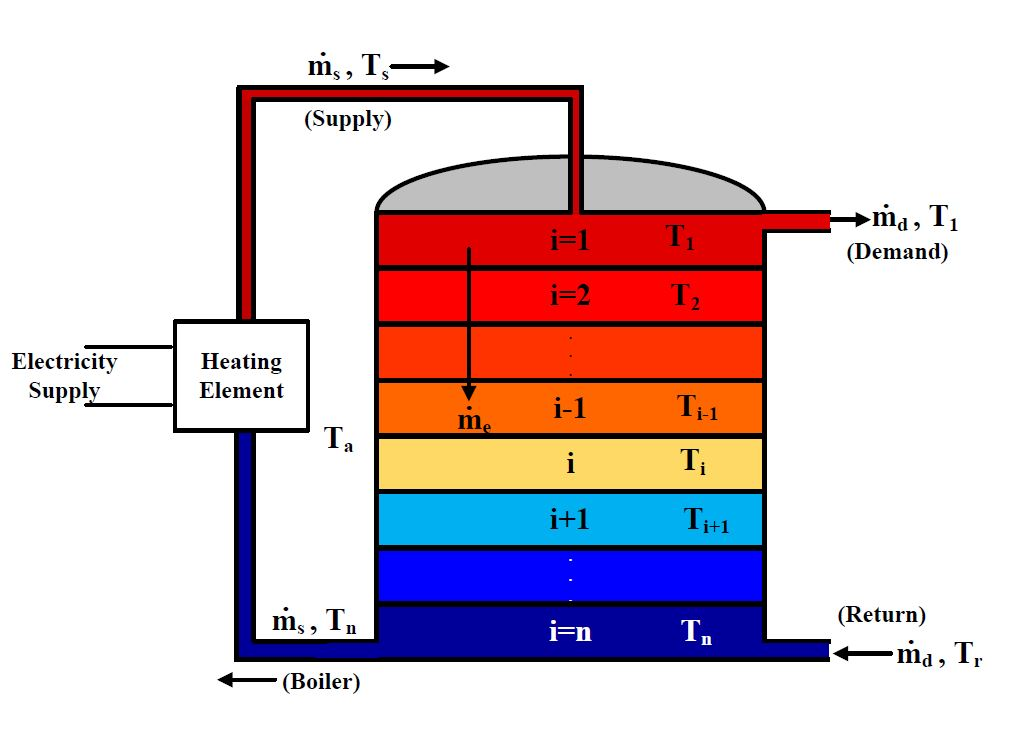
\includegraphics[width=0.8\columnwidth]{Pictures/buffervessel_setup.JPG}
	\caption[Short title]{Buffer vessel representation}
\end{figure}

Due to the fact that the density of water with different temperature layers are created.

In order to model this, the buffervessel will be divided into N-different sections 


\section{Mathematical description}


For the top layer:

\begin{equation}
	\label{eq:Buffer vessel top layer}
	mC_w \dfrac{dT_1}{dt} = \dot{m_s}C_w(T_s - T_1) + \dot{m_e}C_w(T_1 - T_2)*sgn(\dot{-m_e}) - UA_s(T_1 - T_a) - \frac{A_q\lambda_w}{z}(T_1-T_2)
\end{equation}

For the middle layers:

\begin{equation}
	\label{eq:Buffer vessel middle layers}
	mC_w \dfrac{dT_i}{dt} = \dot{m_e}C_w(T_{i-1} - T_{i})*sgn(\dot{m_e}) + \dot{m_e}C_w(T_{i} - T_{i+1})*sgn(\dot{-m_e}) - UA_s(T_i - T_a) + \frac{A_q\lambda_w}{z}(T_{i-1} + T_{i+1} - 2T_i)
\end{equation}

For the bottom layer:

\begin{equation}
	\label{eq:Buffer vessel bottom layer}
	mC_w \dfrac{dT_n}{dt} = \dot{m_d}C_w(T_r - T_n) + \dot{m_e}C_w(T_{n-1} - T_n)*sgn(\dot{m_e}) - UA_s(T_n + T_a) + \frac{A_q\lambda_w}{z}(T_{n-1}-T_n)
\end{equation}

 